Parabolische Koordinaten $(y^1,y^2)$ in der Ebene sind durch die
\index{parabolische Koordinaten}%
Koordinatenabbildung  $\varphi\colon (y^1,y^2)\mapsto (x^1,x^2)$ mit
\begin{align}
x^1 &= y^1y^2
\label{buch:202:eq1}
\\
x^2 &= \frac12\bigl((y^2)^2 - (y^1)^2\bigr)
\label{buch:202:eq2}
\end{align}
gegeben.
\begin{teilaufgaben}
\item 
Finden Sie die Jacobi-Matrix der Abbildung $\varphi$
\item
Finden Sie die Koordinatentransformationsformeln $\psi$, die die
kartesischen Koordinaten $(x^1,x^2)$ in die parabolischen Koordinaten
$(y^1,y^2)=\psi(x^1,x^2)$ umrechnet.
\item
Berechnen Sie die Jacobi-Matrix von $\psi$.
\item
Rechnen Sie nach, dass das Produkt der beiden Matrizen die Einheitsmatrix ist.
\end{teilaufgaben}
\begin{figure}
\centering
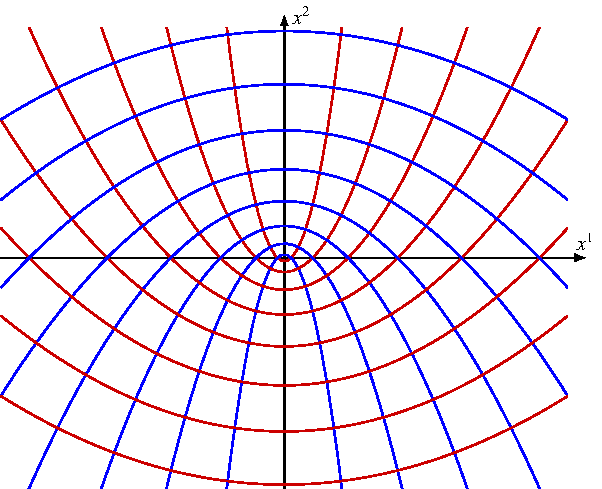
\includegraphics{chapters/020-koordinaten/uebungsaufgaben/parabolisch.pdf}
\caption{Koordinatenlinien für parabolische Koordinaten
\label{202:fig:koordinatenlinien}}
\end{figure}
%

\begin{hinweis}
Berechnen Sie $(x^1)^2+(x^2)^2$.
\end{hinweis}

\begin{loesung}
\begin{teilaufgaben}
\item
Die partiellen Ableitungen sind
\begin{align*}
D\varphi
&=
\bgroup
\renewcommand{\arraystretch}{1.4}
\begin{pmatrix}
\frac{\partial x^1}{\partial y^1}&\frac{\partial x^1}{\partial y^2}\\
\frac{\partial x^2}{\partial y^1}&\frac{\partial x^2}{\partial y^2}
\end{pmatrix}
\egroup
=
\begin{pmatrix}
\phantom{-}y^2 & y^1 \\
         - y^1 & y^2
\end{pmatrix}
\end{align*}
\item
Nach dem Hinweis ist
\begin{align}
(x^1)^2 + (x^2)^2
&=
(y^1y^2)^2
+
\frac14 (y^1)^4 - \frac12 (y^1)^2(y^2)^2 + \frac14 (y^2)^4
\notag
\\
&=
\frac14 (y^1)^4 + \frac12 (y^1)^2(y^2)^2 + \frac14 (y^2)^4
\notag
\\
&=
\biggl(
\frac12\bigl((y^1)^2 + (y^2)^2\bigr)
\biggr)^2.
\\
\sqrt{(x^1)^2+(x^2)^2} &= \frac12\bigl((y^1)^2 + (y^2)^2\bigr)
\label{buch:202:eq3}
\end{align}
Die Gleichungen 
\eqref{buch:202:eq2}
und
\eqref{buch:202:eq3}
können nach $(y^1)^2$ und $(y^2)^2$ aufgelöst werden, indem man
Summe und Differenz der Gleichungen berechnet.
So erhält man
\begin{align*}
&\text{Summe:}
&
\!\sqrt{(x^1)^2+(x^2)^2}
+
x^2
&=
(y^2)^2
&&\Rightarrow&
y^2
&=
\!\sqrt{
\!\sqrt{(x^1)^2+(x^2)^2}
+
x^2
}
\\
&\text{Differenz:}
& 
\!\sqrt{(x^1)^2+(x^2)^2}
-
x^2
&=
(y^1)^2
&&\Rightarrow&
y^1
&=
\!\sqrt{
\!\sqrt{(x^1)^2+(x^2)^2}
-
x^2
}.
\end{align*}
\item
Die Ableitungen der Umkehrabbildung $\psi$ sind
\begin{align*}
D\psi
&=
\frac{1}{
2\!\sqrt{(x^1)^2 +(x^2)^2}
}
\begin{pmatrix}
\displaystyle
\frac{x^1}{
\!\sqrt{\!\sqrt{(x^1)^2+(x^2)^2}-x^2}
}
&
\displaystyle
-\!\sqrt{\!\sqrt{(x^1)^2+(x^2)^2}-x^2}
\\
\displaystyle
\frac{x^1}{
\!\sqrt{\!\sqrt{(x^1)^2+(x^2)^2}+x^2}
}
&
\displaystyle
\phantom{-}\!\sqrt{\!\sqrt{(x^1)^2+(x^2)^2}+x^2}
\end{pmatrix}.
\end{align*}
\item
Um das Produkt der Matrizen $D\psi$ und $D\varphi$ zu berechnen,
drücken wir $D\psi$ mindestens teilweise durch die $y^k$-Koordinaten
aus:
\[
D\psi
=
\frac{1}{
2\!\sqrt{(x^1)^2 +(x^2)^2}
}
\begin{pmatrix}
\displaystyle
\frac{x^1}{y^1}
&
\displaystyle
-y^1
\\
\displaystyle
\frac{x^1}{y^2}
&
\displaystyle
\phantom{-}
y^2
\end{pmatrix}.
\]
Die Einträge in der ersten Spalte können mit \eqref{buch:202:eq1} 
vereinfacht werden zu
\[
D\psi
=
\frac{1}{ 2\!\sqrt{(x^1)^2 +(x^2)^2} }
\begin{pmatrix}
y^2 & -y^1 \\
y^1 & \phantom{-} y^2
\end{pmatrix}.
\]
Damit kann jetzt das Produkt berechnet werden, es ist
\begin{align*}
D\psi\, D\varphi
&=
\frac{1}{ 2\!\sqrt{(x^1)^2 +(x^2)^2} }
\begin{pmatrix}
y^2 & -y^1 \\
y^1 & \phantom{-} y^2
\end{pmatrix}
\begin{pmatrix}
\phantom{-}y^2 & y^1 \\
         - y^1 & y^2
\end{pmatrix}
\\
&=
\frac{1}{ 2\!\sqrt{(x^1)^2 +(x^2)^2} }
\begin{pmatrix}
(y^2)^2+(y^1)^2 & y^2y^1-y^1y^2 \\
y^1y^2 - y^2y^1 & (y^1)^2+(y^2)^2
\end{pmatrix}.
\end{align*}
Die Ausserdiagonalelemente verschwinden, während die
Diagonalelemente wegen \eqref{buch:202:eq3} zu 1 werden.
Es folgt $D\psi\,D\varphi = I$.
\qedhere
\end{teilaufgaben}
\end{loesung}
